
% !TEX encoding = UTF-8 Unicode
% !program = pdflatex

\documentclass[a4paper,11pt]{article}
\usepackage[a4paper,top=38mm,right=16mm,bottom=24mm,left=25mm,head=35mm,foot=15mm]{geometry}
\usepackage{cite}

% language
\usepackage[english,ngerman]{babel}

% font
\usepackage[utf8]{inputenc}
\usepackage[T1]{fontenc}
\usepackage[parfill]{parskip}
\usepackage{soul,rotating}
\usepackage{pdflscape}

\usepackage{helvet}
\renewcommand*\familydefault{\sfdefault}

\linespread{1.25}


% variable definitions
\providecommand{\documenttitle}{Tantal - Das Konfliktmineral der ICT}
\providecommand{\documentauthors}{
  Sebastian Brunner,
  Luca Christen,
  Josef Erben,
  Michel Kern,
  Daniel Milenkovic
  }
\providecommand{\documentdate}{30.09.2018}

% configure title page
\title{
  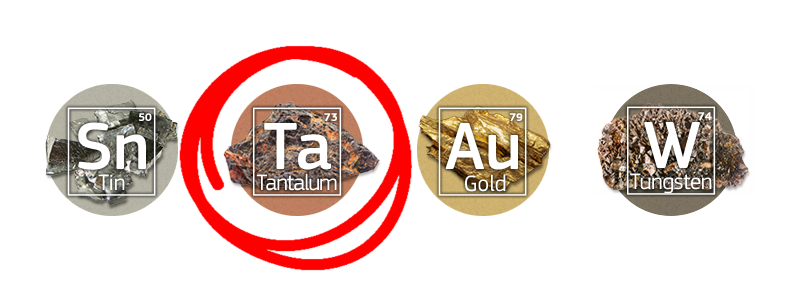
\includegraphics[width=7cm]{images/banner-minerals}\\[\bigskipamount]
  \documenttitle\\[\bigskipamount]
  \large METU 2C Nachhaltigkeit und Informationstechnologien\\[\bigskipamount]
  \large Gruppe D
}
\author{\documentauthors}
\date{\parbox{\linewidth}{\centering%
  Datum \documentdate\endgraf
}}

% table
\usepackage{array}
\usepackage{multicol}
\usepackage{longtable,tabu,booktabs}

% links
\usepackage{hyperref}
\hypersetup{
            pdftitle={\documenttitle},
            pdfauthor={\documentauthors},
            colorlinks=true,
            linkcolor=[RGB]{74,144,226},
            citecolor=[RGB]{74,144,226},
            urlcolor=[RGB]{74,144,226},
            breaklinks=true}
\urlstyle{same}  % don't use monospace font for urls
\newcommand*{\fullref}[1]{\hyperref[{#1}]{\nameref*{#1} (\ref*{#1})}}

% images
\usepackage[font=small,skip=6pt]{caption}
\usepackage{float,graphicx,grffile,wrapfig}
\graphicspath{ {images/} }

\makeatletter
\def\maxwidth{\ifdim\Gin@nat@width>\linewidth\linewidth\else\Gin@nat@width\fi}
\def\maxheight{\ifdim\Gin@nat@height>\textheight\textheight\else\Gin@nat@height\fi}
\makeatother
\setkeys{Gin}{width=\maxwidth,height=\maxheight,keepaspectratio}

\makeatletter
\def\fps@figure{H}
\makeatother

% header and footer
\usepackage{lastpage}
\usepackage{fancyhdr}
\pagestyle{fancy}
\fancyhf{}
\fancyhead[L]{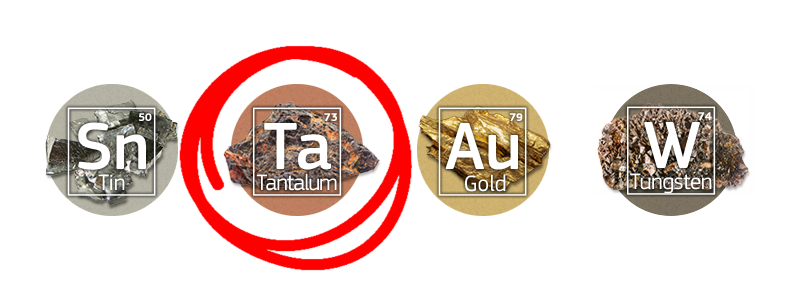
\includegraphics[height=2cm]{images/banner-minerals}}
\fancyfoot[L]{\fontsize{8}{10}\selectfont\ \documenttitle}
\fancyfoot[R]{\fontsize{8}{10}\selectfont\ Seite\ \thepage\ von\ \pageref*{LastPage}}

\renewcommand{\headrulewidth}{0pt}
\renewcommand{\footrulewidth}{0pt}


% headers
\usepackage{titlesec}
% \titlespacing*{\section}{0pt}{1em}{0pt}
% \titlespacing*{\subsection}{0pt}{1em}{0pt}
% \titlespacing*{\subsubsection}{0pt}{1em}{0pt}

\begin{document}

% title page
\maketitle\thispagestyle{empty}\newpage

% abstract page
\selectlanguage{english}
\begin{abstract}
  ~\cite{Nobody06}

Gliederung: Ziel/Aufgabe, Vorgehensweise, Resultate

Lorem ipsum dolor sit amet, consectetur adipiscing elit. Nunc dignissim ultrices sapien eget ornare. Ut facilisis felis a ipsum consequat congue. Pellentesque posuere, massa sed sodales finibus, nisl tortor sollicitudin turpis, sit amet pellentesque libero enim nec est. Sed laoreet mauris ac eros rutrum, rhoncus fringilla tortor pellentesque. Vestibulum viverra porttitor risus, vitae fringilla arcu faucibus vel. Etiam sit amet elit eu orci sodales efficitur. Pellentesque sodales libero vitae dui ullamcorper varius a ultrices turpis. Quisque mi justo, finibus non ullamcorper non, semper sit amet tortor.

Duis a dui nulla. Integer faucibus pretium tellus vel feugiat. Nullam nibh est, tincidunt quis suscipit vel, ultrices sit amet lectus. Sed in aliquet est. Sed tincidunt dignissim magna, at vehicula ex faucibus dapibus. Curabitur tempor dui ac ex pharetra aliquam nec vitae est. Etiam fermentum tempus risus id scelerisque. Mauris ac pellentesque purus. Praesent vel lacus nec eros vestibulum egestas.

Nullam ut scelerisque libero, eget porta nisi. Etiam at porta justo, ac volutpat leo. Suspendisse non vestibulum nibh, eget porta nulla. Lorem ipsum dolor sit amet, consectetur adipiscing elit. Mauris placerat libero eu sagittis molestie. Proin congue libero eget libero venenatis, vestibulum viverra tellus consectetur. Cras pretium faucibus turpis, dapibus condimentum purus maximus ut. Nunc vitae gravida elit. Ut pellentesque viverra neque. Donec vehicula enim sit amet neque venenatis finibus. Curabitur nec faucibus turpis. Donec cursus ex tortor, non euismod diam interdum sed. Sed accumsan leo id accumsan tempor. Proin commodo eleifend sem imperdiet scelerisque.

          \newpage
\end{abstract}
\selectlanguage{ngerman}

% start content
\section{Motivation \& Methodik}\label{sec:motivation}

\subsection{Warum im Tantal interessant?}

In elektronischen Geräten wie Smartphones und Laptops sind Kondensatoren im Einsatz.
Hersteller von Kondensatoren greifen dabei vor allem auf Tantal zurück. Dieses Metall wird aus einem Mineral gewonnen, welches einer der vier Konfliktminerale ist.~\cite{why_tantal}
Förderung und Handel solcher Minerale in Konfliktgebieten können zu schweren Menschenrechtsverletzungen und Verletzungen des humanitären Völkerrechts führen. Oftmals bleibt der Reichtum nicht in den Förderländern.
~\cite{conflict_minerals}

\subsection{Methodik}

Nachfolgend untersuchen wir Tantal aufgrund der häufigen Verwendung in ICT im Kontext der Nachhaltigkeit. Dabei betrachten wir Nachhaltigkeitsindikatoren der Wirtschaft, der Gesellschaft und der Umwelt in 2013 und in 2035. Dies zeigt die Nachhaltigkeit von Tantal bei stetig ansteigendem Bedarf.
Anschliessend zeichnen wir ein alternatives Szenario, bei dem die Nachfrage nach Kondensatoren aus Tantal und somit die Nachfrage durch ICT komplett verschwindet. Dies zeigt den Einfluss der Nachfrage nach Tantal durch ICT auf die Nachhaltigkeit auf.

\subsection{Zielsetzung}

Es werden die Dimensionen Wirtschaft, Gesellschaft und Umwelt für folgende Situationen untersucht:

\paragraph{2013}
Wie war die Situation im Jahr 2013?
\paragraph{2035}
Wie sieht die Situation bei gleichbleibend steigendem Tantalbedarf im Jahr 2035 aus?
\paragraph{2035 (Alternativszenario)}
Durch technolgische Innovation bricht der Bedarf nach Kondensatoren aus Tantal ein. Wie sieht die Situation bei sinkendem Tantalbedarf im Jahr 2035 aus?

\section{Wirtschaftlich}\label{sec:conflict}

* Ausmasse von Zahlen?
* Beteiligte Konzerne
* Abbau vs Recycling?
* Als Output eine Zahl fuer Dimension

Lorem ipsum dolor sit amet, consectetur adipiscing elit. Nunc dignissim ultrices sapien eget ornare. Ut facilisis felis a ipsum consequat congue. Pellentesque posuere, massa sed sodales finibus, nisl tortor sollicitudin turpis, sit amet pellentesque libero enim nec est. Sed laoreet mauris ac eros rutrum, rhoncus fringilla tortor pellentesque. Vestibulum viverra porttitor risus, vitae fringilla arcu faucibus vel. Etiam sit amet elit eu orci sodales efficitur. Pellentesque sodales libero vitae dui ullamcorper varius a ultrices turpis. Quisque mi justo, finibus non ullamcorper non, semper sit amet tortor.

Duis a dui nulla. Integer faucibus pretium tellus vel feugiat. Nullam nibh est, tincidunt quis suscipit vel, ultrices sit amet lectus. Sed in aliquet est. Sed tincidunt dignissim magna, at vehicula ex faucibus dapibus. Curabitur tempor dui ac ex pharetra aliquam nec vitae est. Etiam fermentum tempus risus id scelerisque. Mauris ac pellentesque purus. Praesent vel lacus nec eros vestibulum egestas.

Nullam ut scelerisque libero, eget porta nisi. Etiam at porta justo, ac volutpat leo. Suspendisse non vestibulum nibh, eget porta nulla. Lorem ipsum dolor sit amet, consectetur adipiscing elit. Mauris placerat libero eu sagittis molestie. Proin congue libero eget libero venenatis, vestibulum viverra tellus consectetur. Cras pretium faucibus turpis, dapibus condimentum purus maximus ut. Nunc vitae gravida elit. Ut pellentesque viverra neque. Donec vehicula enim sit amet neque venenatis finibus. Curabitur nec faucibus turpis. Donec cursus ex tortor, non euismod diam interdum sed. Sed accumsan leo id accumsan tempor. Proin commodo eleifend sem imperdiet scelerisque.

\section{Umwelt}\label{sec:solutions}

Im folgenden Kapitel wird der Abbau und die Nutzung von
Tantal und die daraus resultierenden Folgen für die Umwelt untersucht.
Das Hauptaugenmerk liegt dabei auf der Bewertung einzelner Indikatoren im Bezug
auf deren Beitrag zur Nachhaltigkeit.
\subsection{Indikatoren}

\paragraph{Rohstoffverbrauch / Rohstoffbestand}
Dieser Indikator befasst sich mit dem weltweiten Verbrauch des Rohstoffs
Tantal und den Auswirkungen auf dessen globalen Bestand. Ein steigender
Verbrauch beziehungsweise ein sinkender Bestand wird im Bezug auf die
Nachhaltigkeit als negativ eingestuft.

\paragraph{Abbau / Regelung}
Um eine Aussage über die Nachhaltigkeit der Tantalgewinnung machen zu können,
muss der direkte Einfluss des Abbaus auf die Umwelt betrachtet werden. Dabei
soll untersucht werden, welche Methoden dafür angewandt werden und ob diese
risikobehaftet sind, zum Beispiel aufgrund von toxischen Emissionen.

\paragraph{Naturraum / Landschaft}
Massgebend für die Bewertung dieses Indikators ist der Einfluss der
Tantalgewinnung auf den Naturraum im betroffenen Abbaugebiet und die mittel- bis
langfristige Veränderung der Landschaft.

\subsection{Bewertung}
Die globale Fördermenge von Tantal lag \textbf{2013} bei geschätzten 1300 Tonnen. Davon wurden
knapp 40\% für die Herstellung von Kondensatoren verwendet. Prognosen gehen
davon aus, dass sich dieser Bedarf bis ins Jahr \textbf{2035} mehr als
verdoppeln wird ~\cite{Weltweit69:online}.
Zum  weltweiten Bestand lassen sich nur schwer Aussagen machen, da sich ein grosser
Teil des Vorkommens in Konfliktregionen befindet und somit kein kontrollierter
Abbau stattfindet. Das U.S Geological Survey (USGS) geht jedoch davon aus, dass
im Jahr 2018 noch über 110'000 Tonnen an Reserven vorhanden
sind ~\cite{ober2018mineral}.
In Anbetracht des prognostizierten Verbrauches werden ohne Gegenmassnahmen
mittelfristig Engpässe auftreten. Schätzungen darüber, wann dies sein wird,
reichen dabei von 15 bis 125 Jahren ~\cite{behrendt2007seltene}. Durch die Einführung neuer Technologien und dem
damit einhergehenden kompletten Verzicht auf Tantal in der ICT bis zum Jahr \textbf{2035} kann dies
zwar aufgeschoben, jedoch nicht verhindert werden. Dies liegt einerseits daran,
dass auch in anderen Anwendungsgebieten von Tantal mit einem enormen Anstieg des
Verbrauches gerechnet wird. Andererseits werden heute nur ungefähr 10 - 20\%
aller aus Tantal gefertigten Bauteile am Ende ihrer Nutzung recyclet ~\cite{behrendt2007seltene}.

\begin{figure}[h]
\centering
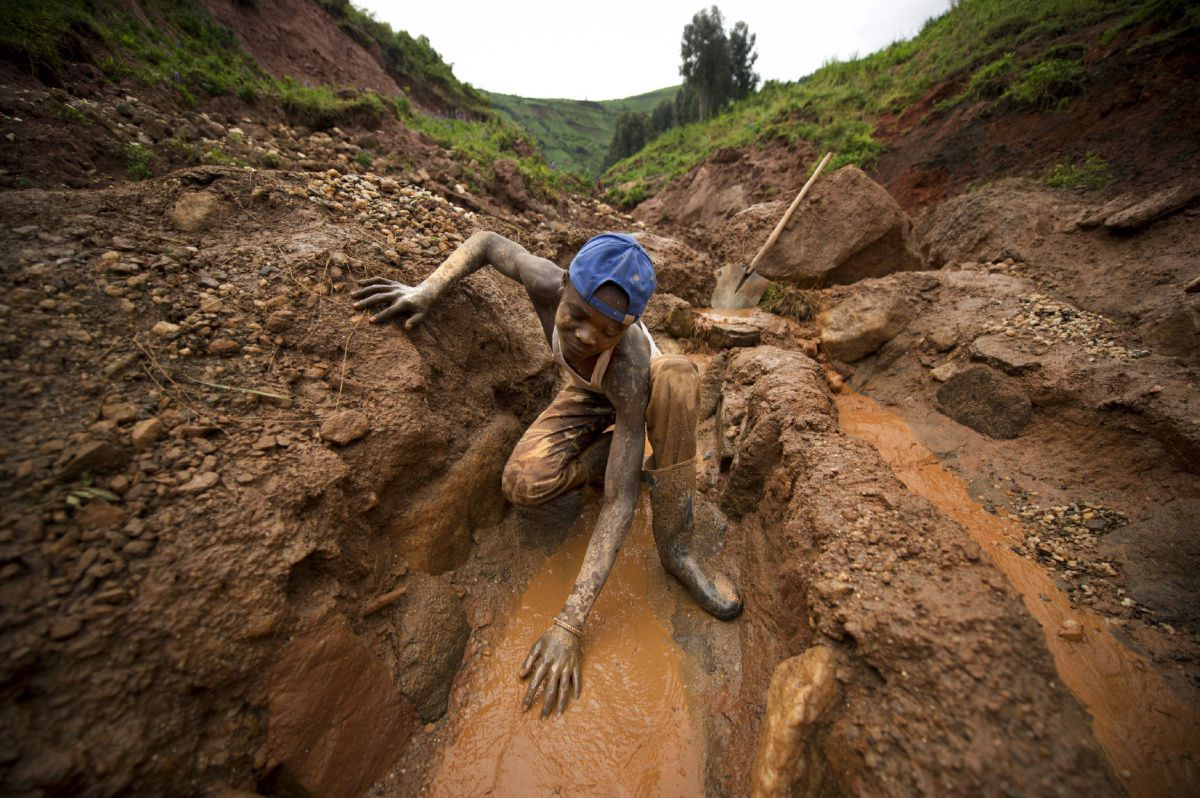
\includegraphics[width=0.8\textwidth]{coltan_in_thecongo1}
\caption{Arbeiter in einer Coltan Mine im Kongo ~\cite{Coltanam17:online}}
\label{}
\end{figure}

Da Tantal in der Natur nicht in reiner Form sondern als Bestandteil verschiedener
Mineralien vorkommt, wobei Coltan (\textbf{Col}umbit-\textbf{Tan}talit) das am
weitesten verbreitete ist, betrachten wir in der Folge den \textbf{Abbau} von Coltan.
Da Coltan in den oberen Gesteinsschichten vorkommt, sind die meisten
Coltan-Minen oberflächlich und die Gewinnung nicht sehr
aufwendig ~\cite{reetsch2008effects}. Ausserdem werden dabei keine toxischen
Stoffe verwendet wie bei anderen Mineralien. Die Tatsache, dass die Förderung
mit einfachen Mitteln möglich ist, führt jedoch auch dazu, dass in den
Konfliktregionen Afrikas viele unkontrollierte Minen entstehen. In diesen meist
unter der Kontrolle von lokalen Milizen betriebenen Minen finden Vorschriften
bezüglich des Umweltschutzes in der Regel keine Beachtung ~\cite{bleischwitz2012coltan}.
Untersuchungen belegen, dass zwar erhöhte Werte von toxischen Stoffen wie Arsen
und Uran im Boden und den Gewässern im Umkreis der Minen messbar sind, diese
jedoch unter den von der WHO festgelegten Grenzwerten ~\cite{environmental_management} liegen.

Ganz im Gegensatz zu den direkten Folgen des Coltan-Abbaus, welche nicht extrem
ins Gewicht fallen bezüglich der Nachhaltigkeit, ziehen die Folgen für den
\textbf{Naturraum} der betroffenen Regionen gravierende Konsequenzen mit sich.
So werden grosse Flächen Wald gerodet, um die Minen zu errichten. Dies führt
dazu, dass die Böden unfruchtbar und anfällig auf Bodenerosionen
werden ~\cite{environmental_management}.

\begin{figure}[h]
\centering
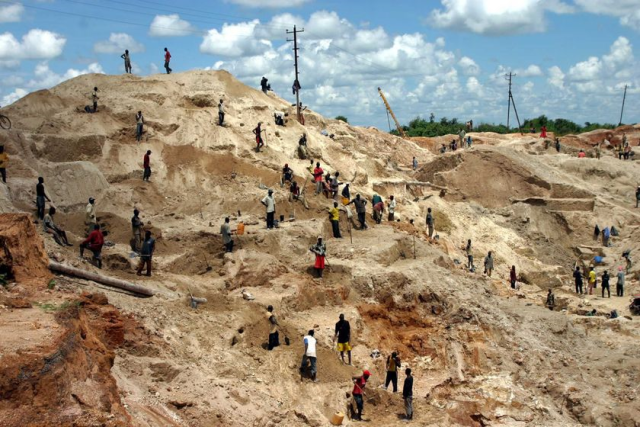
\includegraphics[width=0.8\textwidth]{erosion}
\caption{Bodenerosion verursacht durch Minen ~\cite{Coltanmi34:online}}
\label{}
\end{figure}
\pagebreak

Andererseits liegen viele der Minen der Demokratischen Republik Kongo in
Naturschutzreservaten. Durch die Zerstörung ihres Lebensraumes und die gezielte
Jagd auf die Tiere durch Minenarbeiter verringern sich die Bestände der bereits
vom Aussterben bedrohten Tierarten, wie zum Beispiel dem Berggorilla, dramatisch.
Sollte die Nachfrage nach Tantal tatsächlich so ansteigen wie prognostiziert,
könnte es \textbf{2035} bereits zu spät sein für einige dieser Arten.
Durch den Verzicht auf Tantal durch die ICT-Industrie könnte hier ein wertvoller
Beitrag geleistet werden zur Erhaltung der Artenvielfalt.

\begin{table}[h]
  \centering
  \begin{tabular}{l|ccc}                                    & \textbf{2013} & \textbf{2035} & \textbf{2035 mit Annahme}
    \\ \hline Rohstoffverbrauch / Rohstoffbestand                 & 5             & 2             & 4 
    \\ Abbau / Regelung                                           & 7             & 5             & 6
    \\ Natrurraum / Landschaft                                    & 3             & 2             & 3
    \\ \hline \textbf{Endbewertung}                               & 5             & 3             & 4\(\frac{1}{3}\)
  \end{tabular}
  \caption{Resultat ökologische Analyse}
\end{table}

\section{Gesellschaft}\label{sec:society}

\subsection{Einleitung}

\subsection{Indikatoren}

\subsubsection{Soziale Sicherheit}

Konflikte im Bezug auf Ressourcenabbau.
Finanzierung von Konfliktparteien.

\subsubsection{Gesundheit}

Gesundheit der Minenarbeiter.
Folgen von möglicher Umweltverschmutzung.
Statistiken zu Unfallraten in der Tantalproduktion.

\subsubsection{Solidaritaet}

Gegen die Ausbeutung von armen Laendern.
Bewusstsein der Konsumenten.
Offizielle Massnahmen  z.B. EU etc.

\subsubsection{Chancengleichheit}

Bergbau als Mittel gegen Armut.
Bei hoher Nachfrage höhere Preise -> Australien steigt wieder ein -> Arbeitsplaetze.

\subsection{Bewertung der Indikatoren}

Tabelle mit Bewertung der jeweiligen Indikatoren basierend auf unserer wissenschaftlichen Skala.


@misc{USGSMine8:online,
author = {Désirée E. Polyak},
title = {USGS Minerals Information: Niobium (Columbium) and Tantalum},
howpublished = {\url{https://minerals.usgs.gov/minerals/pubs/commodity/niobium/}},
month = {},
year = {},
note = {(Accessed on 09/13/2018)}
}


\section{Resultate}\label{sec:conflict}

Lorem ipsum dolor sit amet, consectetur adipiscing elit. Nunc dignissim ultrices sapien eget ornare. Ut facilisis felis a ipsum consequat congue. Pellentesque posuere, massa sed sodales finibus, nisl tortor sollicitudin turpis, sit amet pellentesque libero enim nec est. Sed laoreet mauris ac eros rutrum, rhoncus fringilla tortor pellentesque. Vestibulum viverra porttitor risus, vitae fringilla arcu faucibus vel. Etiam sit amet elit eu orci sodales efficitur. Pellentesque sodales libero vitae dui ullamcorper varius a ultrices turpis. Quisque mi justo, finibus non ullamcorper non, semper sit amet tortor.

Duis a dui nulla. Integer faucibus pretium tellus vel feugiat. Nullam nibh est, tincidunt quis suscipit vel, ultrices sit amet lectus. Sed in aliquet est. Sed tincidunt dignissim magna, at vehicula ex faucibus dapibus. Curabitur tempor dui ac ex pharetra aliquam nec vitae est. Etiam fermentum tempus risus id scelerisque. Mauris ac pellentesque purus. Praesent vel lacus nec eros vestibulum egestas.

Nullam ut scelerisque libero, eget porta nisi. Etiam at porta justo, ac volutpat leo. Suspendisse non vestibulum nibh, eget porta nulla. Lorem ipsum dolor sit amet, consectetur adipiscing elit. Mauris placerat libero eu sagittis molestie. Proin congue libero eget libero venenatis, vestibulum viverra tellus consectetur. Cras pretium faucibus turpis, dapibus condimentum purus maximus ut. Nunc vitae gravida elit. Ut pellentesque viverra neque. Donec vehicula enim sit amet neque venenatis finibus. Curabitur nec faucibus turpis. Donec cursus ex tortor, non euismod diam interdum sed. Sed accumsan leo id accumsan tempor. Proin commodo eleifend sem imperdiet scelerisque.



\bibliography{citations}
\bibliographystyle{ieeetran-de}


\end{document}
